
\documentclass[ letterpaper, titlepage, fleqn]{article}

\usepackage[utf8]{inputenc}
\usepackage[slovene]{babel}
\usepackage[margin=60px]{geometry}
\usepackage{amsmath}
\usepackage{amssymb}
\usepackage{enumerate}
\usepackage{graphicx}
\usepackage{mathrsfs}
\usepackage{mathabx}
\setlength\parindent{0pt}

\newcommand{\R}{\mathbb R}
\newcommand{\N}{\mathbb N}
\newcommand{\Z}{\mathbb Z}
\newcommand{\C}{\mathbb C}
\newcommand{\Q}{\mathbb Q}
\newcommand{\F}{\mathscr{F}}
\newcommand{\E}{\mathbb E}
\newcommand{\FF}{\mathbb F}
\newcommand{\K}{\mathbb K}
\newcommand{\D}{\mathbb D}

\newcommand{\mul}{\text{mul}}
\newcommand{\add}{\text{add}}
\newcommand{\abs}{\text{abs}}
\newcommand{\aph}{\text{@}}
\newcommand{\primea}{\textsc{\char13}}
\newcommand{\norm}[1]{\left\lVert#1\right\rVert}
\newcommand{\scalar}[1]{\left\langle#1\right\rangle}
\newcommand{\openbox}{\leavevmode
  \hbox to.77778em{%
  \hfil\vrule
  \vbox to.675em{\hrule width.6em\vfil\hrule}%
  \vrule\hfil}}

\usepackage{tikz}
\usetikzlibrary{calc}
\usetikzlibrary{arrows,decorations.markings}

\tikzset{
    right angle quadrant/.code={
        \pgfmathsetmacro\quadranta{{1,1,-1,-1}[#1-1]}     % Arrays for selecting quadrant
        \pgfmathsetmacro\quadrantb{{1,-1,-1,1}[#1-1]}},
    right angle quadrant=1, % Make sure it is set, even if not called explicitly
    right angle length/.code={\def\rightanglelength{#1}},   % Length of symbol
    right angle length=2ex, % Make sure it is set...
    right angle symbol/.style n args={3}{
        insert path={
            let \p0 = ($(#1)!(#3)!(#2)$) in     % Intersection
                let \p1 = ($(\p0)!\quadranta*\rightanglelength!(#3)$), % Point on base line
                \p2 = ($(\p0)!\quadrantb*\rightanglelength!(#2)$) in % Point on perpendicular line
                let \p3 = ($(\p1)+(\p2)-(\p0)$) in  % Corner point of symbol
            (\p1) -- (\p3) -- (\p2)
        }
    }
}

\begin{document}

\thispagestyle{empty}
\noindent{\large
UNIVERZA V LJUBLJANI\\[1mm]
FAKULTETA ZA MATEMATIKO IN FIZIKO\\[5mm]
\vfill

\begin{center}{\large
Nejc Ševerkar, Matija Šteblaj\\[2mm]
{\bf Spojena kubična Bezierjeva krpa}\\[10mm]
RPGO}
\end{center}
\vfill

\noindent{\large
Ljubljana, 2021}
\pagebreak

\thispagestyle{empty}
\tableofcontents
\pagebreak

\section{Aproksimacijska shema}
Želimo poiskati preprosto $C^1$-ploskev, ki v danih točkah $(x_i, y_i) \in \R^2$, $i=1, \ldots, n$ interpolira predpisane vrednosti in parcialne odvode (npr. od neke funkcije).

Problema se lotimo na sledeč način: naredimo triangulacijo domene na danih točkah in definiramo lokalno shemo na vsakem trikotniku posebej, kjer poskrbimo za ustrezna ujemanja na presekih (skupnih stranicah) trikotnikov. Pri tem si bomo pomagali z Bézierjevimi krpami stopnje 3.

\subsection{Lokalna shema}
Spomnimo se, da je parametrizacija  Bézierjeve krpe stopnje 3 na nekem trikotniku podana s kontrolnimi točkami $b_{ijk}, i+j+k=3$ kot:
\begin{equation}
\label{eq:par}
\begin{split}
	P(u,v,w) =& \sum_{i+j+k=3} b_{ijk} B_{ijk}^3(u,v,w) \\
		=& u^3 \text{ }b_{300} + 3u^2 v \text{ }b_{210} + 3u^2 w \text{ }b_{201} + 3u v^2 \text{ }b_{120}\\
		&+ 3uw^2 \text{ }b_{102} + v^3 \text{ }b_{030} + 3v^2 w \text{ }b_{021} + 3v w^2 \text{ }b_{012} \\
		&+ w^3 \text{ }b_{003} + 6uvw \text{ }b_{111}
\end{split}
\end{equation}
in njen odvod v smeri $\textbf{z} = (z_u,z_v,z_w)$ enak:
\begin{equation}
\label{eq:der}
\frac{\partial{P}}{\partial{\textbf{z}}} = \frac{\partial{P}}{\partial{u}} z_u+ \frac{\partial{P}}{\partial{v}} z_v+ \frac{\partial{P}}{\partial{w}} z_w = \scalar{\text{grad}(P), \textbf{z}}\text{,}
\end{equation}
kjer $u,v,w$ predstavljajo baricentrične koordinate v danem trikotniku.\\

Recimo, da triangulacijo že imamo, in vzemimo nek trikotnik $\scalar{V_1, V_2, V_3}$ v domeni. Določiti moramo točke kontrolne mreže $b_{ijk}$ nad tem trikotnikom:
	\begin{figure}[h]
		\centering
		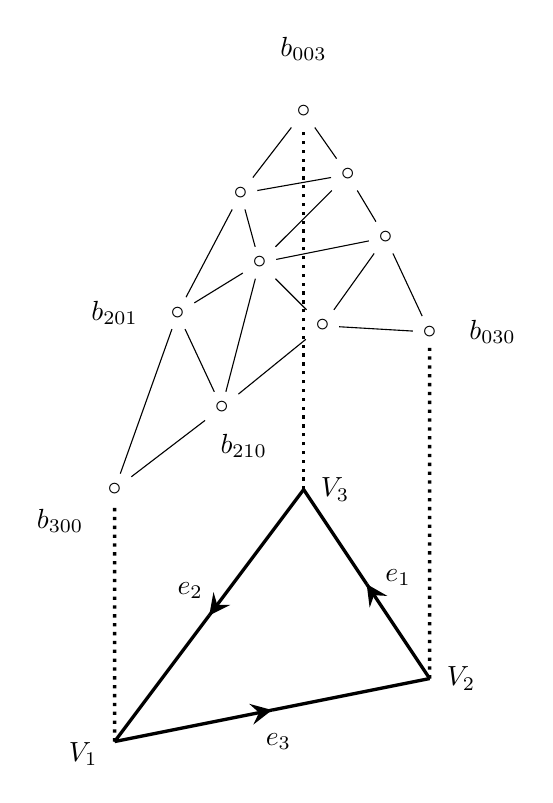
\begin{tikzpicture}[scale=0.8]
			\node (sidro) at (0,0) {};
			
			\node (V1) at ($(sidro)+(-3,-1)$) {};
			\node (p1) at ($(V1) + (-0.5, -0.2)$){$V_1$};
			\node (V15) at ($(V1) + (2.5, 0.5)$){};
			\node (V2) at ($(sidro)+(2,0)$) {};
			\node (p2) at ($(V2) + (0.5, 0)$){$V_2$};
			\node (V25) at ($(V2) + (-1, 1.5)$){};
			\node (V3) at ($(sidro)+(0,3)$) {};
			\node (p3) at ($(V3) + (0:0.5)$){$V_3$};
			\node (V35) at ($(V3) + (-1.5, -2)$){};
			%vektor e_3 = (5,1), e_1 = (-2,3), e_2 = (-3,-4)

			\node (b300) at ($(V1) + (0,4)$){$\circ$};
			\node (300) at ($(b300) + (210:1)$){$b_{300}$};
			\node (b003) at ($(V3) + (0,6)$){$\circ$};
			\node (003) at ($(b003) + (90:1)$){$b_{003}$};
			\node (b030) at ($(V2) + (0,5.5)$){$\circ$};
			\node (030) at ($(b030) + (0:1)$){$b_{030}$};

			\node(b201) at ($(V1) + (1, 1.3) + (0,5.5)$){$\circ$};
			\node(201) at ($(b201) + (180:1)$){$b_{201}$};
			\node(b102) at ($(V1) + (2, 2.7) + (0,6)$){$\circ$};


			\node(b210) at ($(V1) + (1.7, 0.3) + (0,5)$){$\circ$};
			\node(210) at ($(b210) + (300:0.7)$){$b_{210}$};
			\node(b120) at ($(V1) + (3.3, 0.6) + (0,6)$){$\circ$};

			\node(b021) at ($(V2) + (-0.7, 1) + (0,6)$){$\circ$};
			\node(b012) at ($(V2) + (-1.3, 1) + (0,7)$){$\circ$};

			\node(b111) at ($(V1) + (3.3,0.6) + (-1,1.5) +(0,5.5)$){$\circ$};


			\node (e1) at ($(V25) + (0.5,0.1)$){$e_1$};
			\node (e2) at ($(V35) + (-0.3,0.4)$){$e_2$};
			\node (e3) at ($(V15) + (0.1,-0.5)$){$e_3$};


			\draw[very thick, black,decoration={markings,mark=at position 1 with {\arrow[scale=1.5,>=stealth]{>}}},postaction={decorate}] (V1.center) -- (V15.center);
			\draw[very thick, black] (V15.center) -- (V2.center);
			\draw[very thick, black,decoration={markings,mark=at position 1 with {\arrow[scale=1.5,>=stealth]{>}}},postaction={decorate}] (V2.center) -- (V25.center);
			\draw[very thick, black] (V25.center) -- (V3.center);
			\draw[very thick, black,decoration={markings,mark=at position 1 with {\arrow[scale=1.5,>=stealth]{>}}},postaction={decorate}] (V3.center) -- (V35.center);
			\draw[very thick, black] (V35.center) -- (V1.center);

			\draw[very thick, black, dotted] (V1.center) -- (b300);
			\draw[very thick, black, dotted] (V2.center) -- (b030);
			\draw[very thick, black, dotted] (V3.center) -- (b003);

			\draw[black] (b300) -- (b210);
			\draw[black] (b300) -- (b201);

			\draw[black] (b210) -- (b120);
			\draw[black] (b210) -- (b111);
			\draw[black] (b210) -- (b201);

			\draw[black] (b201) -- (b111);
			\draw[black] (b201) -- (b102);

			\draw[black] (b102) -- (b111);
			\draw[black] (b102) -- (b003);
			\draw[black] (b102) -- (b012);

			\draw[black] (b003) -- (b012);

			\draw[black] (b012) -- (b021);
			\draw[black] (b012) -- (b111);

			\draw[black] (b120) -- (b111);
			\draw[black] (b120) -- (b021);

			\draw[black] (b021) -- (b111);

			\draw[black] (b030) -- (b120);
			\draw[black] (b030) -- (b021);

		\end{tikzpicture}
	\end{figure}

Predpisane imamo vrednosti $F(V_i)$ in parcialne odvode $F_x(V_i), F_y(V_i)$ za $V_i = (x_i, y_i)$ $i=1,2,3$. Od tod lahko dobimo odvode v smeri stranic kot:
$$F_{e_i} = \frac{\partial{F}}{\partial{e_i}}  = (x_{i-1}- x_{i+1}) F_x + (y_{i-1}-y_{i+1}) F_y = \scalar{e_i,\text{grad}(F)} \text{,}$$
kjer razumemo $0 \equiv 3$ in $4 \equiv 1$ v indeksih.

S pomočjo teh odvodov lahko definiramo kontrolne točke ``okoli'' enega oglišča trikotnika:
\[
\begin{split}
	b_{300} =& F(V_1) \\
	b_{210} =& F(V_1) + \frac{F_{e_3}}{3} \\
	b_{201} =& F(V_1) - \frac{F_{e_2}}{3}
\end{split}
\]
Opazimo, da s tako izbiro kontrolnih točk $b_{210}$ in $b_{201}$ interpoliramo smerna odvoda v dveh linearno neodvisnih smereh (smereh stranic) nad ogliščem. Sledi, da s tem interpoliramo prve odvode v vseh smereh (v oglišču).

Na analogen način določimo še ostale ``robne'' točke:
	\begin{figure}[h]
		\centering
		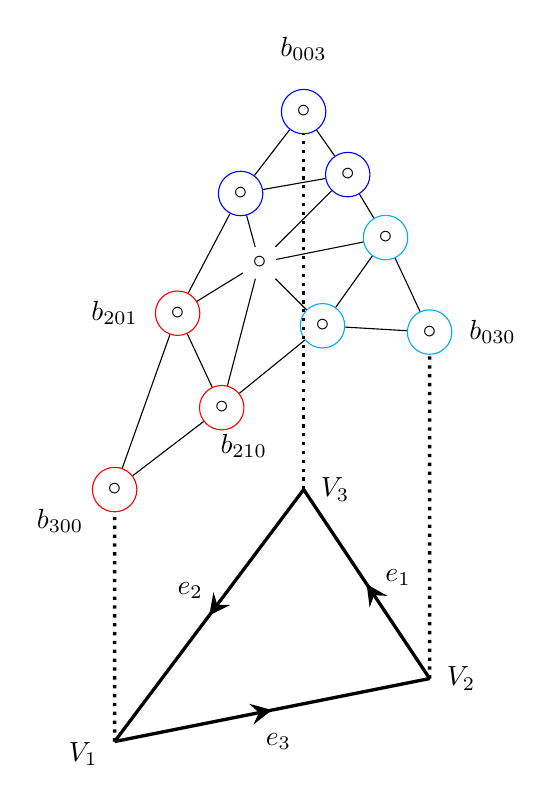
\begin{tikzpicture}[scale=0.8, roundnode/.style={circle, draw=red}, roundnode2/.style={circle, draw=blue}, roundnode3/.style={circle, draw=cyan}]
			\node (sidro) at (0,0) {};
			
			\node (V1) at ($(sidro)+(-3,-1)$) {};
			\node (p1) at ($(V1) + (-0.5, -0.2)$){$V_1$};
			\node (V15) at ($(V1) + (2.5, 0.5)$){};
			\node (V2) at ($(sidro)+(2,0)$) {};
			\node (p2) at ($(V2) + (0.5, 0)$){$V_2$};
			\node (V25) at ($(V2) + (-1, 1.5)$){};
			\node (V3) at ($(sidro)+(0,3)$) {};
			\node (p3) at ($(V3) + (0:0.5)$){$V_3$};
			\node (V35) at ($(V3) + (-1.5, -2)$){};
			%vektor e_3 = (5,1), e_1 = (-2,3), e_2 = (-3,-4)

			\node[roundnode] (b300) at ($(V1) + (0,4)$){$\circ$};
			\node (300) at ($(b300) + (210:1)$){$b_{300}$};
			\node[roundnode2] (b003) at ($(V3) + (0,6)$){$\circ$};
			\node (003) at ($(b003) + (90:1)$){$b_{003}$};
			\node[roundnode3] (b030) at ($(V2) + (0,5.5)$){$\circ$};
			\node (030) at ($(b030) + (0:1)$){$b_{030}$};

			\node[roundnode] (b201) at ($(V1) + (1, 1.3) + (0,5.5)$){$\circ$};
			\node(201) at ($(b201) + (180:1)$){$b_{201}$};
			\node[roundnode2](b102) at ($(V1) + (2, 2.7) + (0,6)$){$\circ$};


			\node[roundnode](b210) at ($(V1) + (1.7, 0.3) + (0,5)$){$\circ$};
			\node(210) at ($(b210) + (300:0.7)$){$b_{210}$};
			\node[roundnode3](b120) at ($(V1) + (3.3, 0.6) + (0,6)$){$\circ$};

			\node[roundnode3](b021) at ($(V2) + (-0.7, 1) + (0,6)$){$\circ$};
			\node[roundnode2](b012) at ($(V2) + (-1.3, 1) + (0,7)$){$\circ$};

			\node(b111) at ($(V1) + (3.3,0.6) + (-1,1.5) +(0,5.5)$){$\circ$};


			\node (e1) at ($(V25) + (0.5,0.1)$){$e_1$};
			\node (e2) at ($(V35) + (-0.3,0.4)$){$e_2$};
			\node (e3) at ($(V15) + (0.1,-0.5)$){$e_3$};


			\draw[very thick, black,decoration={markings,mark=at position 1 with {\arrow[scale=1.5,>=stealth]{>}}},postaction={decorate}] (V1.center) -- (V15.center);
			\draw[very thick, black] (V15.center) -- (V2.center);
			\draw[very thick, black,decoration={markings,mark=at position 1 with {\arrow[scale=1.5,>=stealth]{>}}},postaction={decorate}] (V2.center) -- (V25.center);
			\draw[very thick, black] (V25.center) -- (V3.center);
			\draw[very thick, black,decoration={markings,mark=at position 1 with {\arrow[scale=1.5,>=stealth]{>}}},postaction={decorate}] (V3.center) -- (V35.center);
			\draw[very thick, black] (V35.center) -- (V1.center);

			\draw[very thick, black, dotted] (V1.center) -- (b300);
			\draw[very thick, black, dotted] (V2.center) -- (b030);
			\draw[very thick, black, dotted] (V3.center) -- (b003);

			\draw[black] (b300) -- (b210);
			\draw[black] (b300) -- (b201);

			\draw[black] (b210) -- (b120);
			\draw[black] (b210) -- (b111);
			\draw[black] (b210) -- (b201);

			\draw[black] (b201) -- (b111);
			\draw[black] (b201) -- (b102);

			\draw[black] (b102) -- (b111);
			\draw[black] (b102) -- (b003);
			\draw[black] (b102) -- (b012);

			\draw[black] (b003) -- (b012);

			\draw[black] (b012) -- (b021);
			\draw[black] (b012) -- (b111);

			\draw[black] (b120) -- (b111);
			\draw[black] (b120) -- (b021);

			\draw[black] (b021) -- (b111);

			\draw[black] (b030) -- (b120);
			\draw[black] (b030) -- (b021);

		\end{tikzpicture}
	\end{figure}

Ostane nam le še izbira notranje točke $b_{111}$.\\

 Najprej določimo 3 točke: $b_{111}^1$, $b_{111}^2$, $b_{111}^3$, kjer bo $b_{111}^i$ tak, da bo Bézierjeva krpa s to in prej določenimi kontrolnimi točkami zagotavljala $C^1$-zveznost čez stranico $e_i$. Poglejmo pogoje pri stranici $e_1$, za ostali dve pa naredimo simetrično.
\pagebreak

Poglejmo si notranjo normalo $n_1$ na stranico $e_1$. Velja:
$$n_1 = -e_3 + \frac{e_3 \cdot e_1}{\lvert e_1 \rvert} \frac{e_1}{\lvert e_1 \rvert}$$
\begin{figure}[h]
\centering
		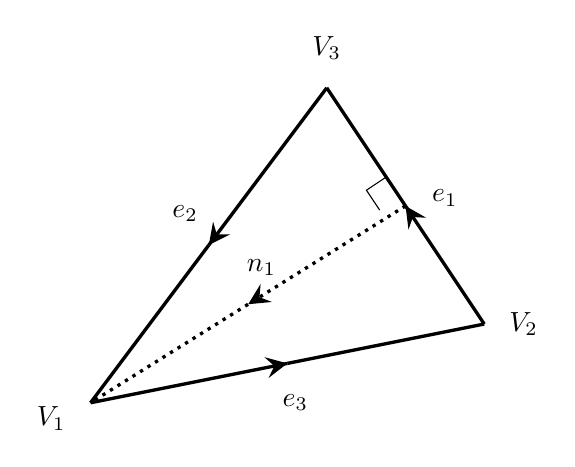
\begin{tikzpicture}
			\node (sidro) at (0,0) {};
			
			\node (V1) at ($(sidro)+(-3,-1)$) {};
			\node (p1) at ($(V1) + (-0.5, -0.2)$){$V_1$};
			\node (V15) at ($(V1) + (2.5, 0.5)$){};
			\node (V2) at ($(sidro)+(2,0)$) {};
			\node (p2) at ($(V2) + (0.5, 0)$){$V_2$};
			\node (V25) at ($(V2) + (-1, 1.5)$){}; %(1,1.5)
			\node (V3) at ($(sidro)+(0,3)$) {};
			\node (p3) at ($(V3) + (0, 0.5)$){$V_3$};
			\node (V35) at ($(V3) + (-1.5, -2)$){};
			%vektor e_3 = (5,1), e_1 = (-2,3), e_2 = (-3,-4), |e_3| / (|e_2| +|e_3|) = ~0.50

			\node (e1) at ($(V25) + (0.5,0.1)$){$e_1$};
			\node (e2) at ($(V35) + (-0.3,0.4)$){$e_2$};
			\node (e3) at ($(V15) + (0.1,-0.5)$){$e_3$};

			\node(H) at ($(V1) + (2, 1.25)$){};
			\node(h) at ($(H) + (70:0.5)$){$n_1$};


			\draw[very thick, black,decoration={markings,mark=at position 1 with {\arrow[scale=1.5,>=stealth]{>}}},postaction={decorate}] (V1.center) -- (V15.center);
			\draw[very thick, black] (V15.center) -- (V2.center);
			\draw[very thick, black,decoration={markings,mark=at position 1 with {\arrow[scale=1.5,>=stealth]{>}}},postaction={decorate}] (V2.center) -- (V25.center);
			\draw[very thick, black] (V25.center) -- (V3.center);
			\draw[very thick, black,decoration={markings,mark=at position 1 with {\arrow[scale=1.5,>=stealth]{>}}},postaction={decorate}] (V3.center) -- (V35.center);
			\draw[very thick, black] (V35.center) -- (V1.center);

			\draw[very thick, black, dotted, decoration={markings,mark=at position 1 with {\arrow[scale=1.5,>=stealth]{>}}},postaction={decorate}] (V25.center)--(H.center);
			\draw[very thick, black, dotted] (H.center)--(V1.center);
			\draw [right angle symbol={V2}{V3}{V1}];

		\end{tikzpicture}
	\end{figure}
	
Če to enačbo razpišemo v baricentričnih koordinatah:
\[
\begin{split}
	n_1 =& -e_3 + \frac{e_3 \cdot e_1}{\lvert e_1 \rvert} \cdot  \frac{e_1}{\lvert e_1 \rvert}\\
		=& -(-1,1,0) - h_1 (0,-1,1) \\
		=& (1,h_1-1,-h_1) \text{,}
\end{split}
\]
kjer je
$$h_1 = -  \frac{e_3 \cdot e_1}{\lvert e_1 \rvert^2}$$
Če označimo s $P_1$ parametrizacijo Bézierjeve krpe , ki jo dobimo iz prej določenih $b_{ijk}$ in $b_{111}^1$, lahko iz formul \ref{eq:par} in \ref{eq:der} izračunamo $\frac{\partial{P_1}}{\partial{n_1}}$. Ta odvod se na stranici $e_1$ (kjer je $u=0$) poenostavi v:
$$\frac{\partial{P_1}}{\partial{n_1}} = 3I_1 v^2 + 6 I_2 vw + 3I_3 w^2 \text{,}$$
kjer so:
\[
\begin{split}
	I_1 &= b_{120}-b_{030}-h_1(b_{021}-b_{030})\\
	I_2 &= b_{111}^1-b_{021}-h_1(b_{012}-b_{021})\\
	I_3 &= b_{102}-b_{012}-h_1(b_{003}-b_{012})
\end{split}
\]

Z upoštevanjem $w=1-v$ (saj je $u+v+w=1$, $u=0$), lahko enačbo preoblikujemo v:
$$\frac{\partial{P_1}}{\partial{n_1}} = 3\bigg((I_1-2I_2+I_3) v^2 + 2 (I_2-I_3) v + I_3 \bigg)$$
Zdaj izberemo tak $b_{111}^1$, da bo ta normalni odvod linearen na stranici $e_1$, tj. linearen v parametru $v$. Dobimo torej enačbo:
$$I_1-2I_2+I_3 = 0$$
Od tod lahko izrazimo:
$$b_{111}^1 = \frac{1}{2}\bigg(b_{120}+b_{102}+h_1(2b_{012}-b_{021}-b_{003}) +(1-h_1)(2b_{021}-b_{030}-b_{012})\bigg)$$

Zakaj taka točka zagotavlja $C^1$ zveznost čez stranico $e_1$? 

Postopek ponovimo na sosednjem trikotniku in dobimo linearen normalen odvod (v nasprotno smer), kar pomeni da je linearen tudi normalen odvod v smeri prvotnega trikotnika. Te dva odvoda se ujemata v ogliščih $V_2$, $V_3$ (shema tam interpolira odvode), torej povsod, ker sta linearna.
\begin{figure}[h]
\centering
		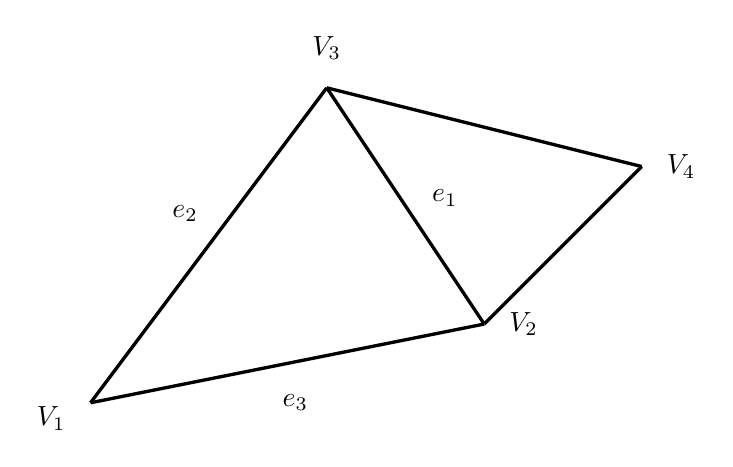
\begin{tikzpicture}%[scale=0.8]
			\node (sidro) at (0,0) {};
			
			\node (V1) at ($(sidro)+(-3,-1)$) {};
			\node (p1) at ($(V1) + (-0.5, -0.2)$){$V_1$};
			\node (V15) at ($(V1) + (2.5, 0.5)$){};
			\node (V2) at ($(sidro)+(2,0)$) {};
			\node (p2) at ($(V2) + (0.5, 0)$){$V_2$};
			\node (V25) at ($(V2) + (-1, 1.5)$){};
			\node (V3) at ($(sidro)+(0,3)$) {};
			\node (p3) at ($(V3) + (0, 0.5)$){$V_3$};
			\node (V35) at ($(V3) + (-1.5, -2)$){};

			\node (V4) at ($(sidro) + (4,2)$){};
			\node(p4) at ($(V4) + (0:0.5)$){$V_4$};
			%vektor e_1 = (5,1), e_2 = (-2,3), e_3 = (-3,-4)

			\node (e1) at ($(V25) + (0.5,0.1)$){$e_1$};
			\node (e2) at ($(V35) + (-0.3,0.4)$){$e_2$};
			\node (e3) at ($(V15) + (0.1,-0.5)$){$e_3$};


			\draw[very thick, black] (V1.center) -- (V2.center);
			\draw[very thick, black] (V2.center) -- (V3.center);
			\draw[very thick, black] (V3.center) -- (V1.center);

			\draw[very thick, black] (V3.center) -- (V4.center);
			\draw[very thick, black] (V2.center) -- (V4.center);


		\end{tikzpicture}
	\end{figure}

\subsection{Celotna shema}

Parametrizacija na celotnem trikotniku bo konveksna kombinacija parametrizacij $P_1$, $P_2$, $P_3$:
\[
\begin{split}
	P(u,v,w) =& \frac{v^2 w^2 P_1 + w^2 u^2 P_2 + u^2 v^2 P_3}{v^2 w^2 + v^2 u^2 + u^2 w^2}\\
		=& u^3 \text{ }b_{300} + 3u^2 v \text{ }b_{210} + 3u^2 w \text{ }b_{201} + 3u v^2 \text{ }b_{120} \\
		&+ 3uw^2 \text{ }b_{102} + v^3 \text{ }b_{030} + 3v^2 w \text{ }b_{021} + 3v w^2 \text{ }b_{012} \\
		&+ w^3 \text{ }b_{003} \\
		&+ 6uvw \frac{v^2 w^2 \text{ } b_{111}^1 + w^2 u^2 \text{ } b_{111}^2 + u^2 v^2 \text{ }b_{111}^3}{v^2 w^2 + v^2 u^2 + u^2 w^2}
\end{split}
\]

Tako definirana parametrizacija se na stranicah ujema z ustrezno lokalno parametrizacijo $P_i$, ki nam zagotavlja $C^1$-zveznost čez stranico $e_i$. Opazimo, da je razlika med našo parametrizacijo in običajno parametrizacijo Bézierjeve krpe le pri točki $b_{111}$, kjer namesto ene točke, ki bi bila fiksna za vse $(u,v,w)$ vzamemo konveksno kombinacijo točk $b_{111}^i$, ki se spreminja z različnimi $(u,v,w)$. Intuitivno si torej lahko predstavljamo, da gre za  Bézierjevo krpo, kjer se notranja točka spreminja z baricentričnimi koordinatami. Ta interpretacija nam tudi omogoča preprosto posplošitev De Casteljaujevega algoritma za izračun točk na naši ploskvi -- za dane parametre najprej izračunamo ustrezen $b_{111}(u,v,w)$, nato izvedemo običajni algoritem.


%%%%%%

\section{Interpolacija razsevnih podatkov v prostoru}
Prejšnjo metodo želimo uporabiti na problemu interpolacije točk $P = (p_i)_{i=1}^n$, kjer je $p_i = (x_i,y_i,z_i) \in \R^3$. 
Mislimo si, da ti podatki ležijo na grafu neke zvezno odvedljive funkcije $f \colon \R^2 \to \R$, ki pa je seveda ne poznamo.
Spomnimo se, da metoda Goodman-Said zahteva poleg vrednosti še poznavanje parcialnih odvodov prvega reda v točkah $(x_i,y_i)_{i=1}^n$.
Ker teh nimamo, jih moramo oceniti.

\subsection{Aproksimacija parcialnih odvodov}
Recimo, da ocenjujemo parcialna odvoda v testni točki $p_k \in P$ (natančneje sta to parcialna odvoda $f$ v $(x_k,y_k)$). 
To bomo storili v treh korakih.

\begin{enumerate}
\item Za oceno odvoda v $p_k$  bomo seveda potrebovali neke informacije o vrednostih $f$ 
v točkah blizu $(x_k,y_k)$. Vse kar imamo na voljo so točke $(x_i,y_i)$, torej izmed njih
izberemo tiste, ki so $(x_k,y_k)$ dovolj blizu. To naredimo z izborom radija $r_k$ in obravnavo točk $p_j \in P$, 
za katere velja
$$d((x_j,y_j), (x_k,y_k)) = d^k_j \in (0, r_k].$$
Označimo množico indeksov teh z $J_k$.
\item Ker tudi med izbranimi točkami prioritiziramo tiste, ki so naši testni točki bližje,
jih ustrezno utežimo. Za $j \in J_k$ definiramo
$$w^k_j := \frac{r_k - d^k_j}{r_k \cdot d^k_j},$$
utež točke $p_j$ glede na $p_k$. 
\item Za $p_k$ definirajmo interpolacijski polinom druge stopnje kot
$$p(x,y) := z_k + a (x - x_k)^2 + b (x - x_k) \cdot (y - y_k) + c (y - y_k)^2 + d (x-x_k) + e(y-y_k),$$
kjer so $a,b,c,d,e \in \R$ nedoločeni koeficienti in velja 
$$p_x(x_k,y_k) = d \quad \text{in} \quad p_y(x_k,y_k) = e.$$
Ti vrednosti bosta oceni za parcialna odvoda v točki $p_k$.
Da bo to smiselno, mora ta polinom v okolici $(x_k,y_k)$ dobro aproksimirati vrednosti funkcije $f$, 
torej vrednosti $z_j$ v točkah $(x_j,y_j)$ za $j \in J_k$.
Če upoštevamo še uteži posamezne točke, so vrednosti določene z minimizacijskim problemom
$$\sum_{j\in J_k} (w^k_j \cdot (p(x_j,y_j) - z_j))^2 = \norm{W_k Au - W_k v}^2,$$
kjer so za $J_k = \{j_1, j_2, \dots, j_{n_k}\}$ \\
\begin{equation*}
\begin{aligned}
W_k = &
\begin{bmatrix}
w_{j_1}^k &  &  &  \\
& w_{j_2}^k &  &  \\
& & \ddots & \\
&  &  & w_{j_{n_k}}^k
\end{bmatrix},
\quad
v = 
\begin{bmatrix}
z_{j_1}- z_k \\
z_{j_2} - z_k \\
\vdots  \\
z_{j_{n_k}} - z_k
\end{bmatrix}, \quad
u =
\begin{bmatrix}
a \\
b \\
c \\
d \\
e
\end{bmatrix} \quad \text{in} \\[6pt]
A =&
\begin{bmatrix}
(x_{j_1}- x_k)^2 &  (x_{j_1} - x_k) \cdot (y_{j_1} - y_k) & (y_{j_1} - y_k)^2 & (x_{j_1} - x_k) & (y_{j_1} - y_k) \\
(x_{j_2} - x_k)^2 & (x_{j_2} - x_k) \cdot (y_{j_2} - y_k) & (y_{j_2} - y_k)^2 & (x_{j_2} - x_k) & (y_{j_2} - y_k) \\
\vdots & \vdots & \vdots & \vdots & \vdots \\
(x_{j_{n_k}} - x_k)^2 & (x_{j_{n_k}} - x_k) \cdot (y_{j_{n_k}} - y_k) & (y_{j_{n_k}} - y_k)^2 & (x_{j_{n_k}} - x_k) & (y_{j_{n_k}} - y_k) \\
\end{bmatrix}
\end{aligned}
\end{equation*} 
Seveda to rešujemo z metodo najmanjših kvadratov, kjer pa moramo predpostaviti,
da je točk znotraj radija dovolj, torej $|J_k| \geq 5$ (to lahko zagotovimo z implicitno
definicijo radija $r_k$, ki ga definiramo kot razdalja od $n$-te najbližje točke za $n\geq 6$).
\end{enumerate}

\begin{figure}[h]
\begin{center}
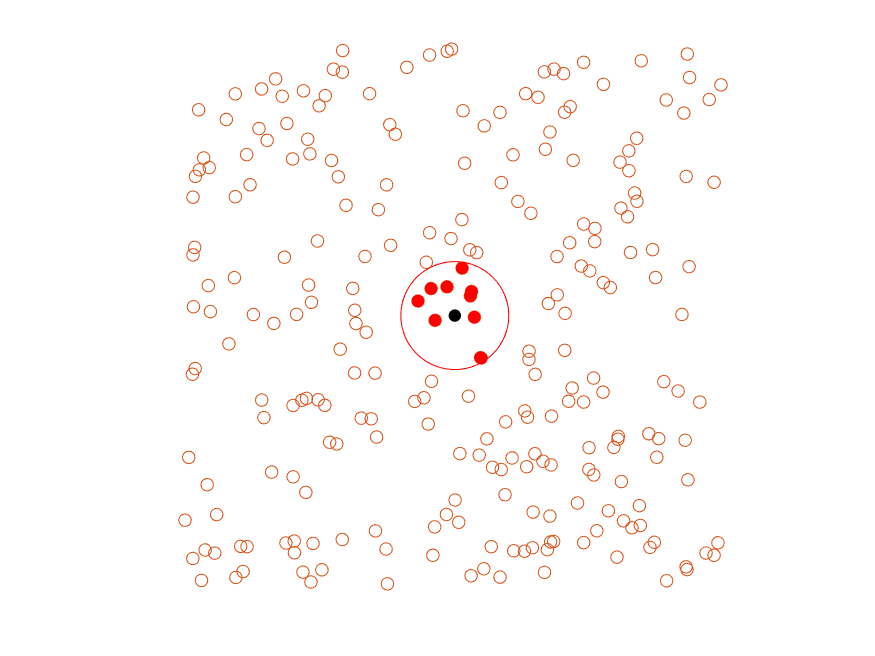
\includegraphics[width=7cm]{slike/derivativeest1.png}
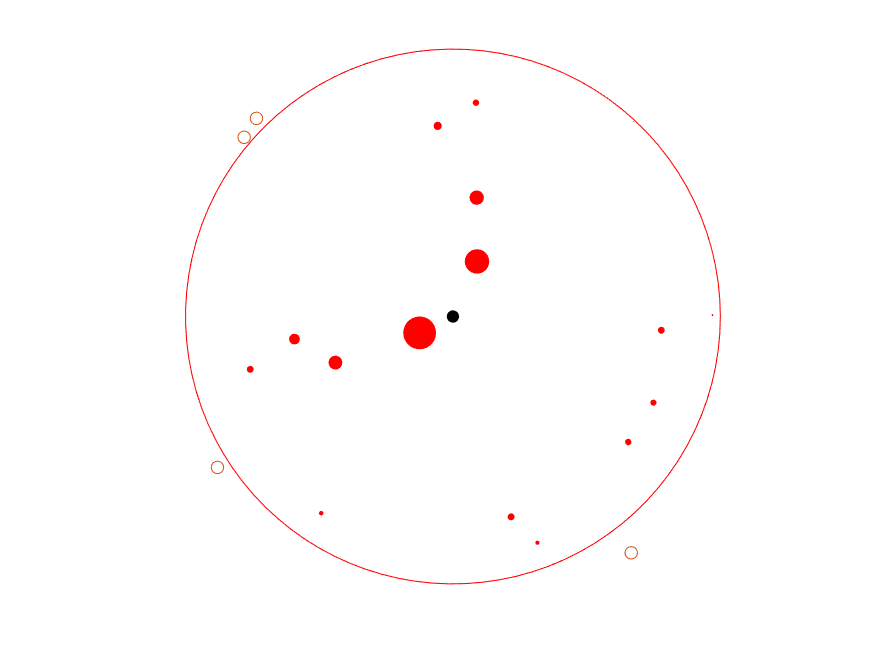
\includegraphics[width=7cm]{slike/derivativeest2.png} 
\end{center} 
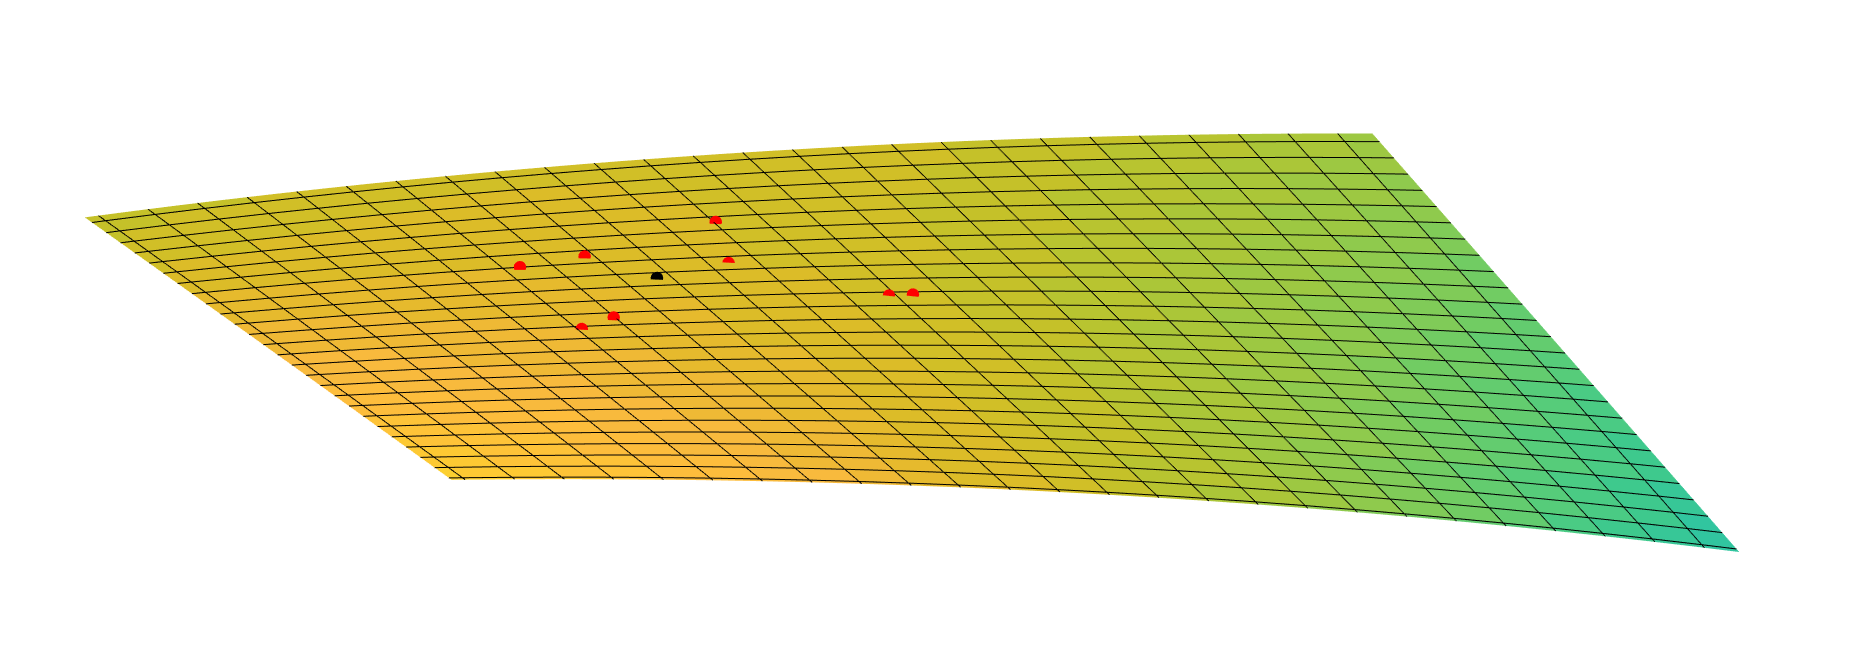
\includegraphics[width=\textwidth]{slike/derivativeest4.png}
\caption{ Trije koraki aproksimacije parcialnih odvodov.}
\end{figure}

\subsection{Postopek}
Sedaj lahko opišemo postopek interpolacije točk v $P$, ki poteka v treh korakih
\begin{enumerate}
\item V vsaki točki $p_k \in P$ ocenimo parcialne odvode.
\item Trianguliramo točke $(x_i,y_i)_{i=1}^n$ z neko triangulacijsko metodo.
\item Na vsakem trikotniku $T$ konstruiramo lokalno shemo z metodo Goodman-Said in shranimo matriko 
koeficientov, definiranih v prvem poglavju
\begin{equation*}
B_T = 
\begin{vmatrix}
b_{300} & b_{210} & b_{120} & b_{030} \\
b_{201} & \openbox & b_{021} & \openbox  \\
b_{102} & b_{012} & \openbox & b_{1112} \\
b_{003} & \openbox & b_{1113} & b_{1111}
\end{vmatrix}
\end{equation*}
\end{enumerate}
Seznam  matrik $B_T$ nad vsakem trikotniku $T$ triangulacije, skupaj z njo
definirajo naš zlepek.

\section{Rezultati implementacije}

\begin{figure}[h]
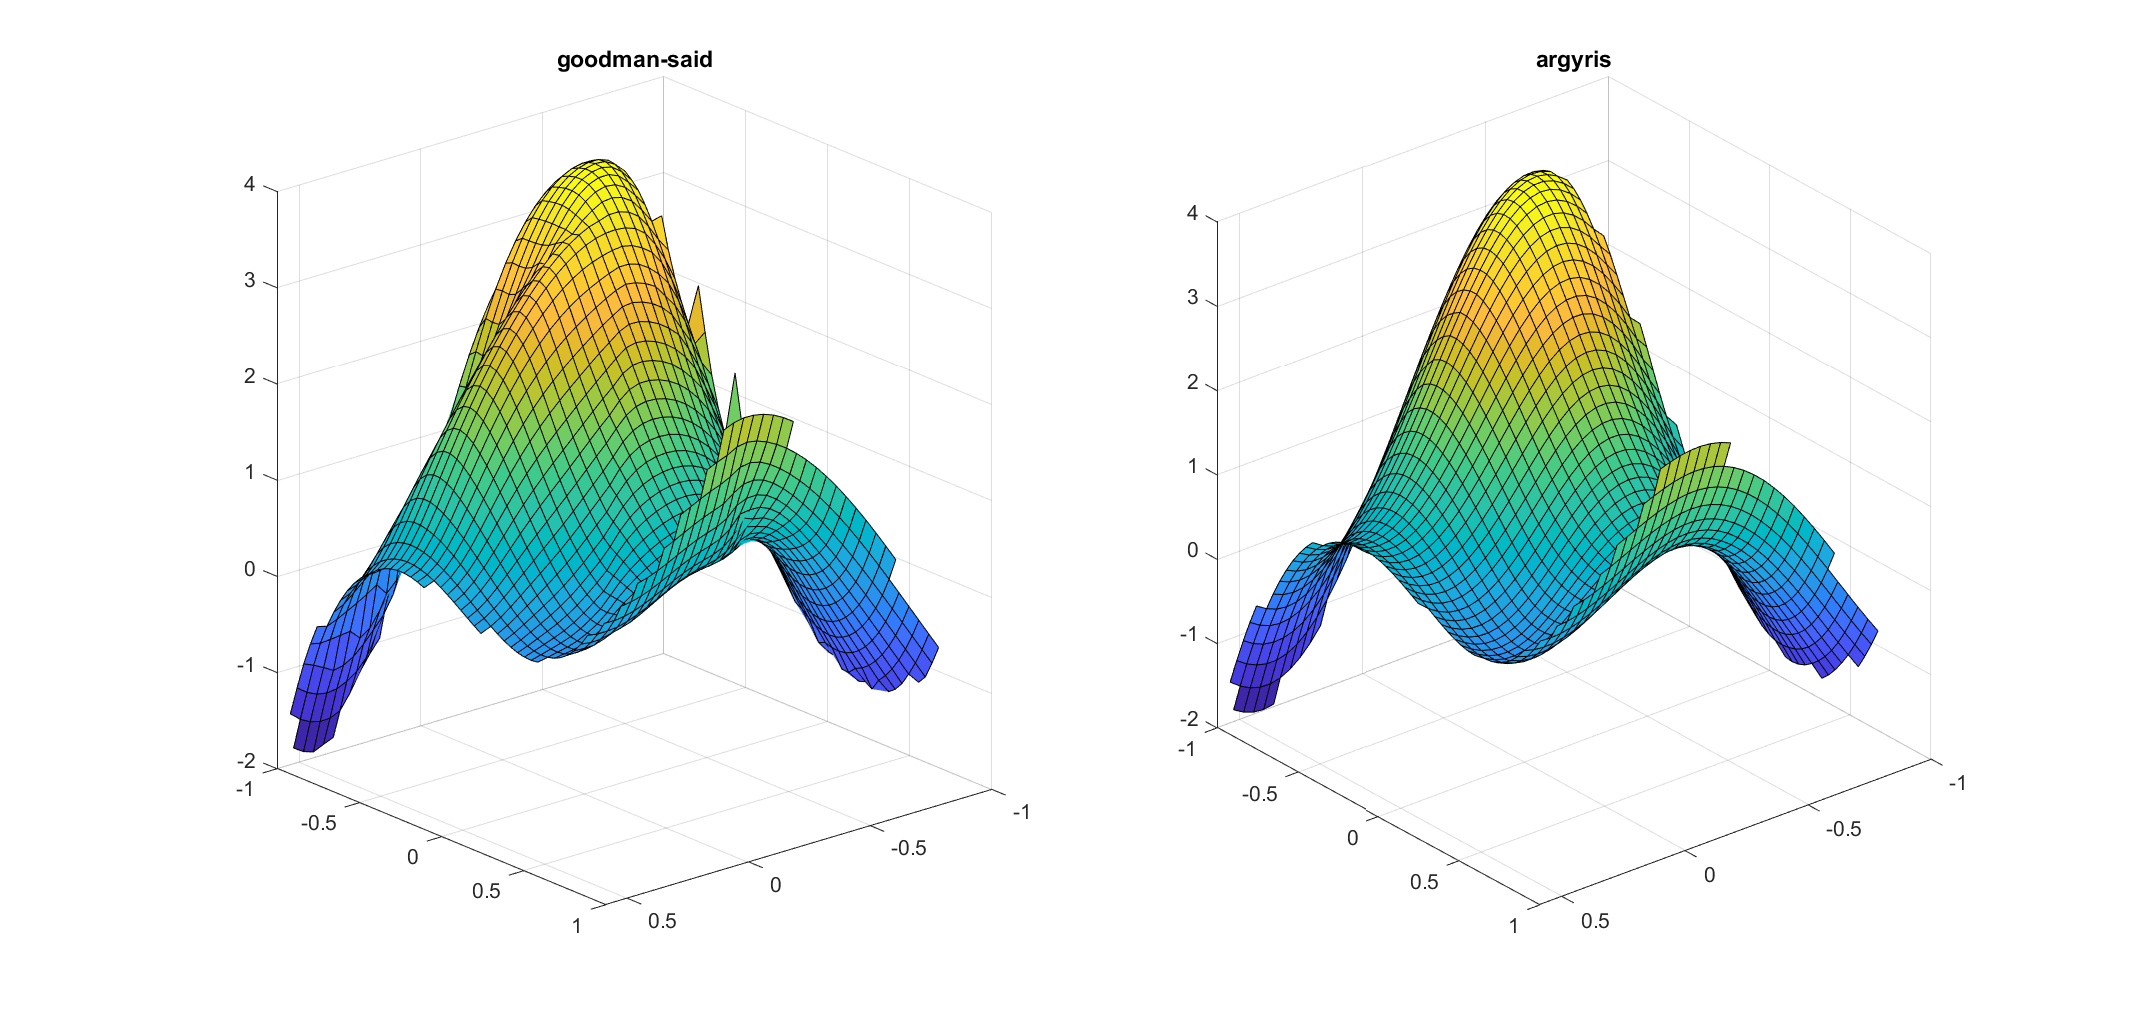
\includegraphics[width=\textwidth]{slike/goodmansaid-vs-argyris.png}
\caption{ 
Primerjava aproksimacije funkcije s shemo Goodman-Said (na levi) in Argyris (na desni),
pri znanih odvodih na $10$-ih točkah. Vidimo, da je Argyrisova shema bolj natančna,
a je pri problemu interpolacije točk v prostoru manj primerna, 
saj moramo za njeno uporabo oceniti poleg prvih še druge parcialne odvode.
}
\end{figure}

\begin{figure}[h]
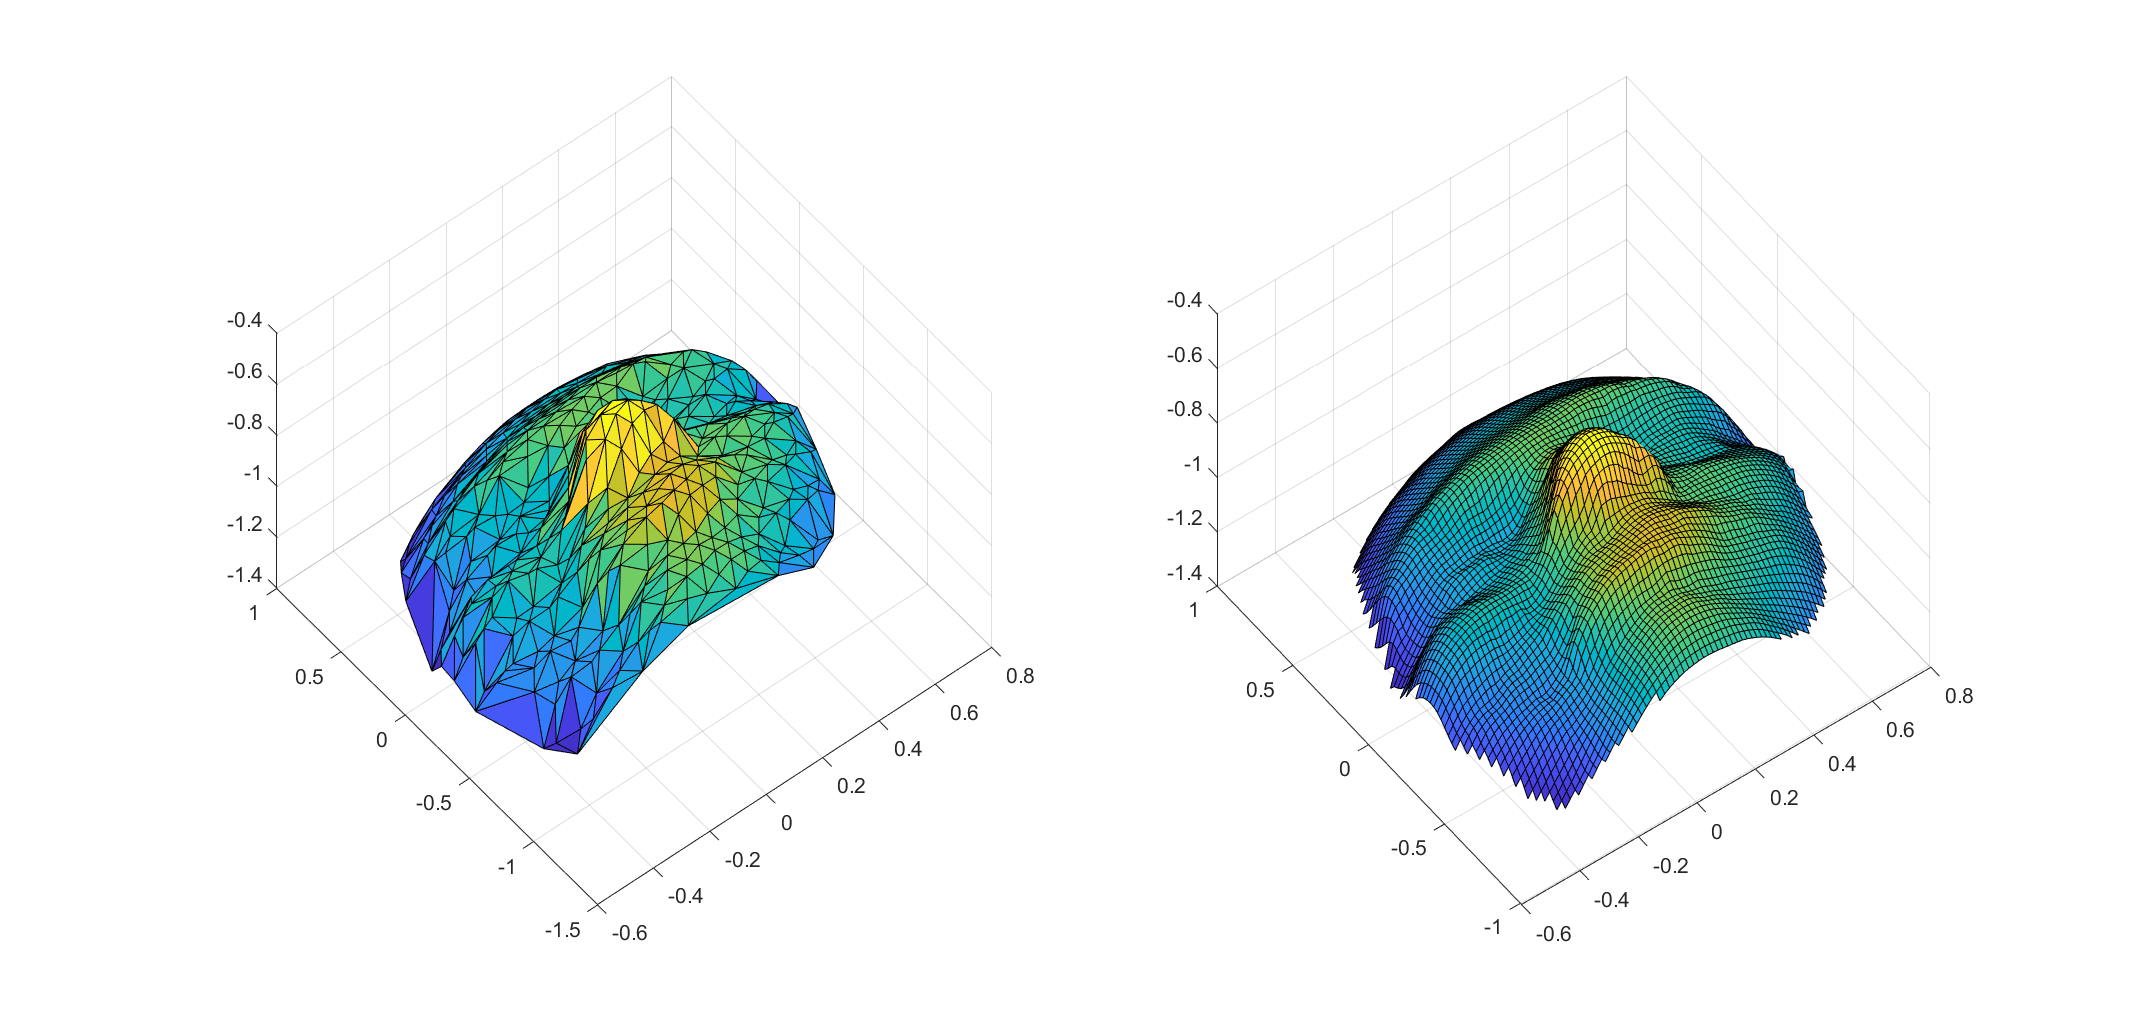
\includegraphics[width=\textwidth]{slike/goodmansaid-face.png}
\caption{ Interpolacija točk v prostoru s shemo Goodman-Said. }
\end{figure}

\begin{figure}[h]
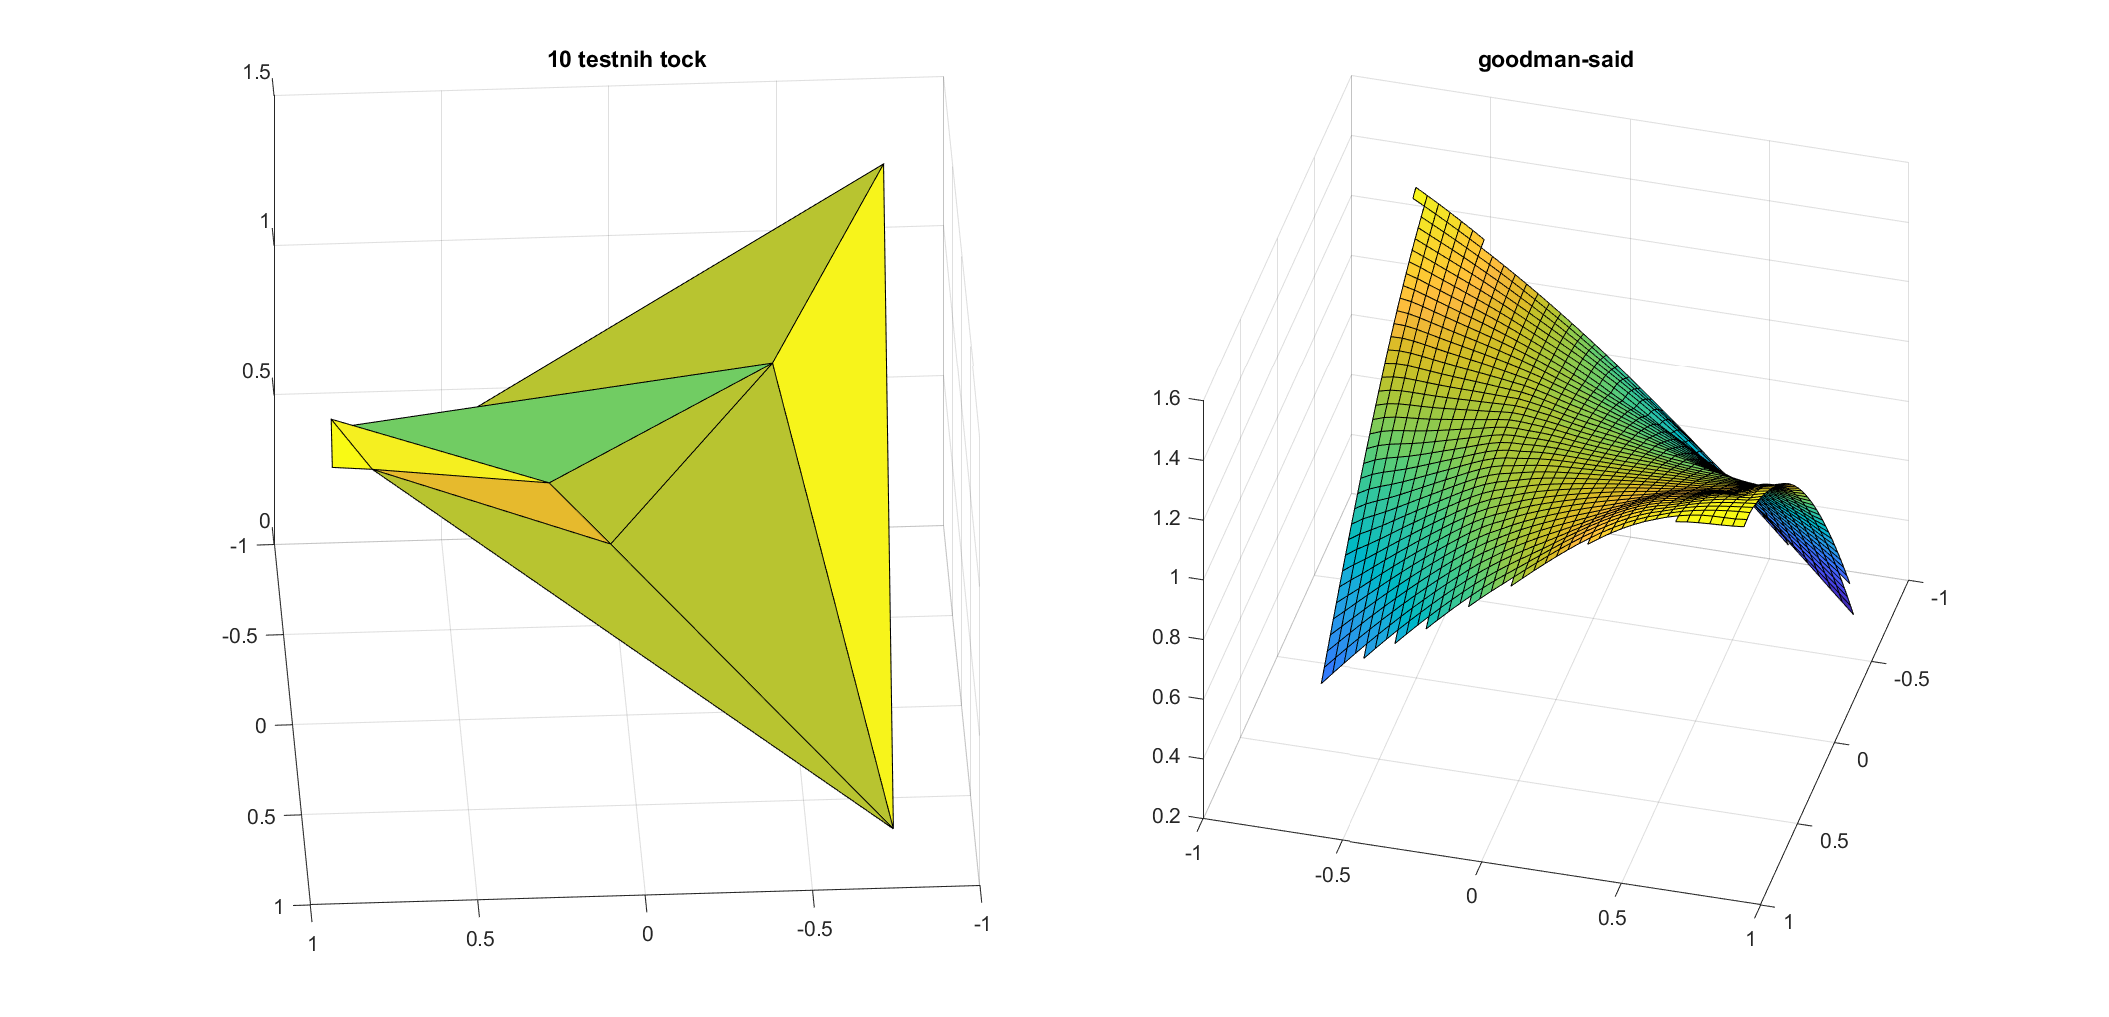
\includegraphics[width=\textwidth]{slike/goodmansaid.png}
\caption{ 
Interpolacija $10$-ih točk na grafu $(x,y) \mapsto \sin(x\cdot y) + \cos(x \cdot y)$ 
s shemo Goodman-Said.
}
\end{figure}

\end{document}
